% one_way_relu.tex — One-Way-Trained ReLU: error correction that only revives.
% Ruach Tov Collective (Heath Hunnicutt & Bocher), November 2026.
% House style: ruachtov.sty. Build: pdflatex one_way_relu.tex (twice for refs).
\documentclass[11pt]{article}
\usepackage{ruachtov}
\renewcommand{\rtproject}{Backpropagation}
\rtdate{16 November 2026}
%% lint: ignore-metaphor{dying ReLU}
%% lint: ignore-metaphor{dead/live}
%% lint: ignore-metaphor{``Dead'' is casually violent}
%% lint: ignore-metaphor{dead tissue}
%% lint: ignore-metaphor{resurrecting the dead}
%% lint: ignore-metaphor{The literature calls this ``dying}
%% lint: ignore-metaphor{a ``dead'' unit}
%% lint: ignore-metaphor{the dead.}
\usepackage[margin=1in]{geometry}
\usepackage{tikz}
\usetikzlibrary{positioning,decorations.pathreplacing,patterns}
\usepackage{circuitikz}
\usepackage{pgfplots}
\pgfplotsset{compat=1.18}
\usepackage{graphicx}
\usepackage{float}
\usepackage{caption}
\newcounter{lstcounter}
\renewcommand{\thelstcounter}{\arabic{lstcounter}}
\usepackage{fancyvrb}
\usepackage{mdframed}
%% codelisting: boxed, kept-together program listing with the caption
%% INSIDE the frame and an en-space of inner margin (Heath's spec).
%% mdframed holds verbatim + caption in one unbreakable frame
%% (nobreak=true); fancyvrb Verbatim supplies the verbatim engine
%% (frame off — the outer mdframed box is the frame now).
\newenvironment{codelisting}[2]{%
  \refstepcounter{lstcounter}#1%
  \par\vspace{0.8\baselineskip}%
  \begin{mdframed}[nobreak=true,
     innerleftmargin=0.5em, innerrightmargin=0.5em,
     innertopmargin=0.5em, innerbottommargin=0.5em,
     skipabove=0.5\baselineskip, skipbelow=0.5\baselineskip,
     linewidth=0.4pt]%
  {\textbf{Listing~\thelstcounter:} #2\par}%
  \vspace{-6pt}\noindent\rule{\linewidth}{0.4pt}\par
  \vspace{-4pt}\small}{%
  \end{mdframed}}

\newcommand{\relu}{\mathrm{ReLU}}
%% Model names, house style (\textsc, as \sortingNetworks in ruachtov.sty).
%% NOTE: the testbed is NOT LeNet-5 (5x5 convs, 6/16 ch, avgpool, tanh,
%% ~60k params) — it is the PyTorch-examples MNIST CNN lineage (3x3,
%% 32/64 ch, maxpool, ReLU, ~1.2M params), so it gets an honest name:
\newcommand{\modelEmnistNet}{\textsc{EmnistNet}\xspace}
\newcommand{\modelCifarNet}{\textsc{CifarNet}\xspace}
\newcommand{\dd}{\mathrm{d}}

\begin{document}

\rttitle{One-Way-Trained ReLU}{Error correction that only revives: a sign-gated backward convention for rectified units}
\author{\sffamily Heath Hunnicutt\thanks{With Bocher and other AI Agents of Ruach Tov Collective (\texttt{https://ruachtov.ai}).}\\[2pt]\normalsize CS576, Purdue University Fort Wayne}
\date{November 2026 --- draft v0.1}
\maketitle

\begin{abstract}
We introduce \emph{one-way-trained ReLU} (``one-way''), a backward-pass
convention for rectified linear units in which correction gradients reach
inactive units only when the error signal favors their revival. The forward
pass is exactly $\relu$; inference is bit-identical. On EMNIST-Balanced
(47 classes, small CNN, $n{=}50$ paired seeds), one-way improves final
accuracy over both plain ReLU ($+0.41$ points, paired $t{=}9.70$, 46/50
seed wins) and standard leaky ReLU ($+0.40$, $t{=}9.63$), improves expected
calibration error by 40\%, and concentrates its gains in the dataset's
confusable character families ($0{\to}O$ errors $-9\%$, $F{\to}f$ $-20\%$).
The advantage is optimizer-independent ($+0.37$ under momentum-SGD, $+0.40$
under Adam), and the method's single hyperparameter is insensitive across
nearly an order of magnitude under both optimizers. Unexpectedly, we find
that Adam itself is a major \emph{driver} of unit squelching (39.5\% of
penultimate-layer units squelched under Adam vs.\ 4.5\% under SGD for plain
ReLU), and that with one-way in place, momentum-SGD matches or exceeds Adam
on this testbed --- suggesting that part of adaptive optimization's benefit
has been compensation for a repairable convention in the backward pass.
The method was verified to the bit level: we emit fused forward and backward
kernels from declarative specifications, prove them 0-ULP against the
autograd reference on CPU and GPU, and document three signed-zero
conventions --- including a previously uncharacterized bit-level divergence
between torch-CPU and torch-GPU at $\relu(-0.0)$.
\end{abstract}

\section{Background}

\subsection{The rectified linear unit}

The rectifier $\relu(x) = \max(x, 0)$ is the dominant activation
nonlinearity of the deep-learning era: cheap, sparse, and free of the
saturation that troubled sigmoid-family units
(Figure~\ref{fig:relu}).

\begin{figure}[H]
\centering
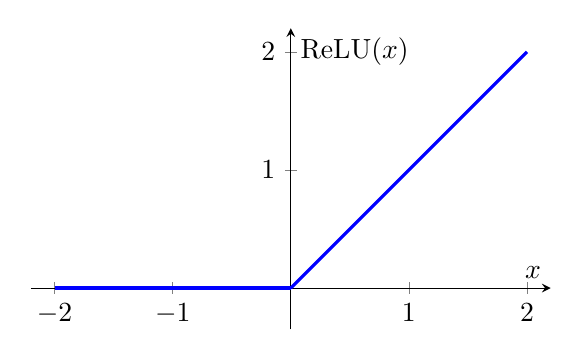
\begin{tikzpicture}
\begin{axis}[
    width=6.6cm, scale only axis, unit vector ratio=1 1,
    axis lines=middle, xlabel=$x$, ylabel={$\relu(x)$},
    xmin=-2.2, xmax=2.2, ymin=-0.35, ymax=2.2,
    xtick={-2,-1,0,1,2}, ytick={1,2},
    samples=2, every axis plot/.append style={very thick}]
\addplot[domain=-2:0, blue] {0};
\addplot[domain=0:2, blue] {x};
\end{axis}
\end{tikzpicture}
\hspace{1.2em}
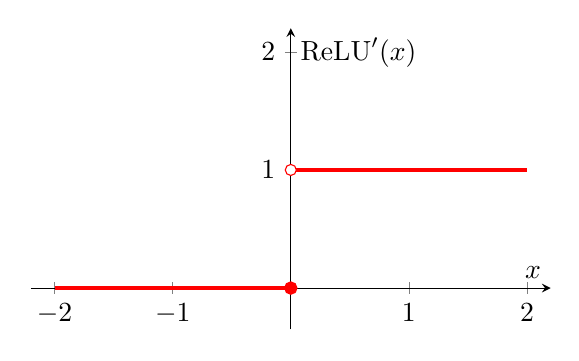
\begin{tikzpicture}
\begin{axis}[
    width=6.6cm, scale only axis, unit vector ratio=1 1,
    axis lines=middle, xlabel=$x$, ylabel={$\relu'(x)$},
    xmin=-2.2, xmax=2.2, ymin=-0.35, ymax=2.2,
    xtick={-2,-1,0,1,2}, ytick={1,2},
    samples=2, every axis plot/.append style={very thick}]
\addplot[domain=-2:-0.03, red] {0};
\addplot[domain=0.03:2, red] {1};
\addplot[red, mark=*, mark size=1.8, only marks] coordinates {(0,0)};
\addplot[red, mark=*, mark size=2.0,
         mark options={fill=white, draw=red, line width=0.4pt},
         only marks] coordinates {(0,1)};
\end{axis}
\end{tikzpicture}

\caption{\emph{Left:} the rectifier's transfer function on
$x \in (-2, 2)$. \emph{Right:} its derivative, drawn to the
\emph{same scale} (square lattice both panels): the derivative is
literally a choice between $0$ and $1$. At $x{=}0$ the function is
nonsmooth and the value $\relu'(0)$ is a \emph{convention}, not a
consequence --- the open circle marks the subtracted point.}
\label{fig:relu}
\end{figure}

\begin{figure}[H]
\centering
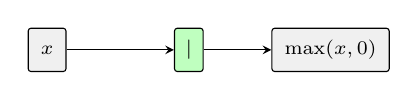
\begin{tikzpicture}[x=0.9cm,
  tens/.style={draw, rounded corners=1pt, fill=gray!12,
               minimum height=5.5mm, inner xsep=1.6mm, font=\scriptsize},
  dio/.style={draw, rounded corners=1pt, fill=green!25,
              minimum height=5.5mm, inner xsep=1.4mm, font=\scriptsize},
  >=stealth]
\node[tens] (x) at (0,0) {$x$};
\node[dio]  (d) at (2,0) {$\blacktriangleright|$};
\node[tens] (y) at (4,0) {$\max(x,0)$};
\draw[->] (x) -- (d);
\draw[->] (d) -- (y);
\end{tikzpicture}
\caption{\textbf{The rectifier as a compute node.} In the compute-graph
figures of this paper, the green node with the diode glyph
$\blacktriangleright|$ depicts the $\relu$ operation --- a one-way
valve (the physical analogy of Section~1.2) as an abstract node
between activation records.}
\label{fig:diodenode}
\end{figure}

\subsection{A physical analogy}

The intuition behind this work is an analog computer's version of the same
circuit (Figure~\ref{fig:circuit}). Consider a potentiometer whose wiper
spans $\pm 5$\,V, feeding an idealized diode (a precision rectifier):

\begin{figure}[h]
\centering
\begin{circuitikz}[american, scale=0.9, transform shape]
  \draw (0,3) node[left]{$+5$\,V} to[short] (1,3)
        to[pR, name=P] (1,0) to[short] (0,0) node[left]{$-5$\,V};
  \node at (1.9,1.6) {wiper};
  \draw (1,1.5) to[short] (3,1.5)
        to[D, l=$D$] (5,1.5)
        to[short] (5.6,1.5) node[circ]{} to[short] (6,1.5)
        to[R, l=$R_L$] (7.6,1.5);
  \draw (7.6,1.5) to[short] (7.6,0.4) node[ground]{};
  \draw (5.6,1.5) to[short] (5.6,2.4) node[above]{$v_{\mathrm{out}}$};
\end{circuitikz}

\caption{The analog-computer rectifier. The dial position is the
pre-activation $x$; the diode clamps $v_{\mathrm{out}}$ at zero
whenever the wiper sits below ground --- but the dial's authority is
independent of the clamp.}
\label{fig:circuit}
\end{figure}

The observation that motivates everything that follows: when the wiper sits
at $-2$\,V, the output is clamped to zero --- but \emph{the dial still
works}. Turning it toward positive voltage acts at full scale, $1{:}1$;
the control path's authority is independent of the clamp. The standard
backward convention $\relu'(x{\le}0) = 0$ models the \emph{transfer
function's} slope. It does not model the \emph{control loop} --- the
mechanism by which correction could re-engage the unit. An embodied
intuition from circuit-building, applied to a formalism that had quietly
conflated the two.

\subsection{The squelched-unit problem}
\label{sec:squelched}

A unit whose pre-activation is negative for every training input receives
zero gradient under the standard convention and can never recover: the
inactive state is \emph{absorbing}. The literature calls this ``dying
ReLU''; in this paper we deliberately say a unit is \emph{squelched}
(vs.\ \emph{included}) --- the choice of vocabulary is deliberate
(Section~\ref{sec:terminology}). Squelched
units are lost capacity: in our EMNIST testbed, plain ReLU under Adam
squelches 30--45\% of the 128 penultimate fully-connected units by epoch
ten.

Standard mitigations assign a small conductance to the inactive side.
\emph{Leaky ReLU}~\cite{maas2013leaky} uses $f(x) = x$ for $x > 0$ and $\alpha x$ otherwise
(typically $\alpha \approx 0.01$), so gradient always flows; \emph{PReLU}~\cite{he2015prelu}
makes $\alpha$ a learned parameter. Both alter the \emph{forward} function
--- inference changes --- and both propagate correction \emph{in either
direction}: a leaky unit can be pushed deeper into inactivity by the same
channel that could revive it.

Bertoin et al.\ \cite{bertoin2021} studied the hidden freedom directly:
treating the value of $\relu'(0)$ as a tunable quantity, they found it
can change training trajectories materially (especially at half
precision), writing that ``algorithmic differentiation of nonsmooth
[functions] potentially hides parameters that could be tuned
advantageously.'' The present work takes that observation one step
further: not only the value \emph{at} the kink, but the \emph{sign
structure of the entire inactive half-line}, is a hidden, tunable
convention.

\subsection{A proposed secondary change to long-standing physical
analogies}
\label{sec:terminology}

Alongside the primary proposal of this paper, we propose a secondary
one, about language: replacing the ``dead/live'' vocabulary of the
rectifier literature with \emph{squelched/included}. We have adopted
the new terminology throughout this paper, for the convenience of all
contributors. Squelch is the radio operator's term: a gate
that mutes a channel whose signal falls below threshold --- mechanical,
reversible in principle, and carrying no connotation of loss beyond the
signal's current absence. ``Dead'' is casually violent, and the metaphor
misleads precisely where this paper works: a ``dead'' unit under the
standard convention is not dead tissue but a \emph{muted channel whose
control path still functions} --- as the potentiometer analogy makes
physical. Thinking ``included vs.\ squelched'' keeps the analysis
mechanical: the engineering problem is lost computational capacity, and
it admits engineering solutions. We also note, writing as a human--AI
collaboration, that clinical vocabulary helps every kind of analyst ---
human or artificial --- maintain the dispassionate stance the problem
deserves; there is more joy in un-muting a channel than in resurrecting
the dead.

\section{One-way-trained ReLU}

\subsection{Definition and motivation}

One-way keeps the forward pass exactly $\relu$. The backward pass is
gated by the \emph{sign of the incoming error}. With upstream gradient
$g = \partial L / \partial y$ (torch convention: $g < 0$ means the loss
decreases if the unit's output increases):
\[
\frac{\partial L}{\partial x} \;=\;
\begin{cases}
g, & x > 0 \quad\text{(included: full gradient)}\\[2pt]
\alpha\, g, & x \le 0 \ \text{and}\ g < 0 \quad\text{(revival direction: leak)}\\[2pt]
0, & x \le 0 \ \text{and}\ g \ge 0 \quad\text{(suppression direction: blocked)}
\end{cases}
\]
with $\alpha \approx 0.01$. The motivation is stated simply: \emph{do not
propagate correction information to neurons that did not participate in
the activation} --- unless that correction would recruit them
(the squelched-unit problem, Section~\ref{sec:squelched}). A squelched
unit contributed nothing to the output; blaming it (pushing it further
negative) teaches nothing, but inviting it (when the ensemble needs more
activation) is constructive. The backward pass becomes itself a rectifier,
oriented opposite the forward one: correction flows one way, toward
inclusion. At $x{=}0$ exactly, this rule coincides with the minimizing
choice over the Clarke subdifferential $[0,1]$ of $\relu$; for $x < 0$ it
is a finite-step (straight-through-style) estimator of where a gradient
step could move the unit.

\textbf{What the rule does and does not guarantee.} The gate is a
filter on the \emph{instantaneous, per-sample} gradient signal: for
an inactive unit it passes an incoming gradient only when that
gradient, taken alone, points in the direction that would increase
the unit's activation. It guarantees nothing about the
\emph{trajectory}. The parameter update that follows aggregates many
such per-sample, per-path signals across the batch, and a stateful
optimizer folds in information from earlier steps --- Adam's moment
estimates or SGD's momentum can carry a revival-signed gradient into
a step that nonetheless moves the pre-activation further negative
(or vice versa). So the actual pre-activation is not guaranteed to
increase, to cross zero, or to remain active once revived; the rule
only ensures that the \emph{suppression} direction receives no fresh
per-sample reinforcement through the gated site. Our measurements
bear the distinction out: under Adam, revival-step magnitudes are
set almost entirely by the optimizer's normalization rather than by
$\alpha$ (Section~\ref{sec:sgd}), and the unit-level telemetry of
the companion program finds 30--35\% of revived units re-silencing
at least once --- revival is a statistical tendency the convention
makes available, not a monotone escape.

\subsection{Interaction with optimizer conditioning}

Bertoin et al.\ observed that Adam and batch normalization \emph{buffer}
the influence of the $\relu'(0)$ choice --- with those reconditioners in
place, varying the convention matters less. Both~\cite{kingma2015adam,ioffe2015bn} can be viewed loosely as
\emph{smoothers of the training signal}: Adam maintains exponential moving
averages of each parameter's gradient (first moment) and squared gradient
(second moment), scaling steps by their ratio, so a parameter's effective
step is normalized by its own recent history; batch normalization
standardizes each layer's pre-activations across the batch, recentering
the operating point of every unit each step. Our measurements
(Section~\ref{sec:sgd}) sharpen the buffering story in an unexpected
direction: Adam's normalization not only buffers the convention --- it
amplifies squelching-side dynamics, and is itself a major source of the
pathology one-way removes.

\section{EMNIST results}
\label{sec:results}

Testbed: EMNIST-Balanced~\cite{cohen2017emnist} (47 character classes, 112{,}800 train /
18{,}800 test), \modelEmnistNet: conv32--conv64--pool--fc128--fc47 ($\approx$1.2M
parameters, PyTorch~\cite{paszke2019pytorch} examples lineage~\cite{lecun1998mnist}, dropout removed to leave
squelching dynamics unconfounded), batch 128, ten epochs, fp32
throughout. All comparisons are \emph{paired}: seed $k$ produces
bit-identical initial weights and identical batch order in every arm
(verified by direct tensor comparison), controlling for initialization
luck. Statistics below use $n{=}50$ seeds per arm.

\subsection{The \modelEmnistNet network: a compute graph}
\label{sec:network}

The testbed network is specified as declarative facts in the
collective's BPD system; the dimension checker \emph{verifies} the
graph (deriving every tensor shape from the input through op semantics
and comparing against declarations), the diagram emitters \emph{draw}
it, and the kernel foundry \emph{compiles} its operators --- one graph,
many projections, with figure captions calculated from the same facts
the verifier checked. Listing~\ref{lst:arch} gives the complete
specification:

\begin{codelisting}{\label{lst:arch}}{\textbf{\modelEmnistNet as
Logtalk program code.} op/4 compute-graph facts encode tensor flow;
per-site modifiers include the backprop-convention facts.}
\begin{Verbatim}
op(c1,      conv2d(1, 32, 3),   [img],  [f_c1]).
op(act_c1,  activation(relu),   [f_c1], [a_c1]).
op(c2,      conv2d(32, 64, 3),  [a_c1], [f_c2]).
op(act_c2,  activation(relu),   [f_c2], [a_c2]).
op(pool,    max_pool2d(2),      [a_c2], [p_c2]).
op(flat_op, flatten,            [p_c2], [flat]).
op(f1,      linear(9216, 128),  [flat], [f_f1]).
op(act_f1,  activation(relu),   [f_f1], [a_f1]).
op(f2,      linear(128, 47),    [a_f1], [logits]).

backprop_convention(act_c1, one_way).
backprop_convention(act_c2, one_way).
backprop_convention(act_f1, one_way).
\end{Verbatim}
\end{codelisting}

The \texttt{backprop\_convention/2} facts make the experimental arm an
explicit, declared property of each activation site --- the arms of
this paper differ \emph{only} in those three facts (the complete
inter-arm diff is printed in the Appendix, Listing~\ref{lst:armdiff}).
Build state for the emitted kernels is itself tracked as facts (the
collective's \texttt{fused\_kernel\_status} schema), so the pipeline
is declarative end to end: graph facts $\to$ emission $\to$ 0-ULP
verification $\to$ build provenance. Shape inference
confirms all ten declared tensors and counts 1{,}204{,}655 parameters,
matching the PyTorch module exactly; Figure~\ref{fig:zigzag} shows
the verified graph as the alternating memory/compute transit the
hardware actually performs.

\begin{figure}[H]
\centering
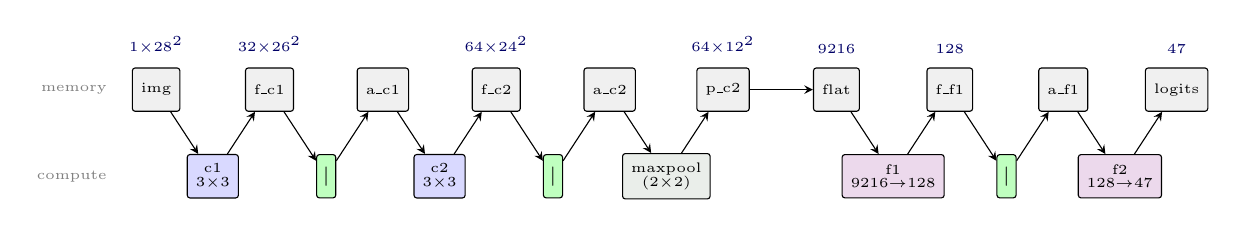
\begin{tikzpicture}[x=0.72cm,
  tens/.style={draw, rounded corners=1pt, fill=gray!12,
               minimum height=5.5mm, inner xsep=1.1mm, font=\tiny},
  opb/.style={draw, rounded corners=1pt, fill=blue!15,
              minimum height=5.5mm, inner xsep=1.1mm, font=\tiny},
  dio/.style={draw, rounded corners=1pt, fill=green!25,
              minimum height=5.5mm, inner xsep=0.8mm, font=\scriptsize},
  dim/.style={font=\tiny, text=blue!40!black},
  >=stealth]
%% ZIGZAG MODE: memory row (top) and ground row (computations, bottom);
%% data alternates: tensor \searrow op \nearrow tensor \searrow op ...
\node[tens] (img)  at (0,0)   {img};
\node[opb, align=center]  (c1)   at (1,-1.1) {c1\\[-1pt]{\tiny $3{\times}3$}};
\node[tens] (fc1)  at (2,0)   {f\_c1};
\node[dio]  (d1)   at (3,-1.1) {$\blacktriangleright|$};
\node[tens] (ac1)  at (4,0)   {a\_c1};
\node[opb, align=center]  (c2)   at (5,-1.1) {c2\\[-1pt]{\tiny $3{\times}3$}};
\node[tens] (fc2)  at (6,0)   {f\_c2};
\node[dio]  (d2)   at (7,-1.1) {$\blacktriangleright|$};
\node[tens] (ac2)  at (8,0)   {a\_c2};
\node[opb, fill=green!10!gray!15, align=center]  (pl)   at (9,-1.1) {maxpool\\[-1pt]{\tiny $(2{\times}2)$}};
\node[tens] (pc2)  at (10,0)  {p\_c2};
\node[tens] (flt)  at (12,0)  {flat};
\node[opb, fill=violet!15, align=center]  (f1)   at (13,-1.1) {f1\\[-1pt]{\tiny $9216{\to}128$}};
\node[tens] (ff1)  at (14,0)  {f\_f1};
\node[dio]  (d3)   at (15,-1.1) {$\blacktriangleright|$};
\node[tens] (af1)  at (16,0)  {a\_f1};
\node[opb, fill=violet!15, align=center]  (f2)   at (17,-1.1) {f2\\[-1pt]{\tiny $128{\to}47$}};
\node[tens] (lg)   at (18,0)  {logits};
%% the zigzag:
\draw[->] (img) -- (c1);
\draw[->] (c1) -- (fc1);
\draw[->] (fc1) -- (d1);
\draw[->] (d1) -- (ac1);
\draw[->] (ac1) -- (c2);
\draw[->] (c2) -- (fc2);
\draw[->] (fc2) -- (d2);
\draw[->] (d2) -- (ac2);
\draw[->] (ac2) -- (pl);
\draw[->] (pl) -- (pc2);
\draw[->] (pc2) -- (flt);
\draw[->] (flt) -- (f1);
\draw[->] (f1) -- (ff1);
\draw[->] (ff1) -- (d3);
\draw[->] (d3) -- (af1);
\draw[->] (af1) -- (f2);
\draw[->] (f2) -- (lg);
%% dims above shape-changing tensors:
\node[dim, above=0.5mm of img] {$1{\times}28^2$};
\node[dim, above=0.5mm of fc1] {$32{\times}26^2$};
\node[dim, above=0.5mm of fc2] {$64{\times}24^2$};
\node[dim, above=0.5mm of pc2] {$64{\times}12^2$};
\node[dim, above=0.5mm of flt] {$9216$};
\node[dim, above=0.5mm of ff1] {$128$};
\node[dim, above=0.5mm of lg]  {$47$};
%% row labels:
\node[font=\tiny, anchor=east, text=gray] at (-0.7, 0)    {memory};
\node[font=\tiny, anchor=east, text=gray] at (-0.7, -1.1) {compute};
\end{tikzpicture}
\caption{\textbf{The \modelEmnistNet compute graph.} (Diode nodes
as introduced in Figure~\ref{fig:diodenode}.) Memory row above,
compute row at ground; the data flows left to right alternating
between them --- img descends into c1, rises as f\_c1, descends
through the diode, rises as a\_c1, and so on: every arrow is a
transit between a computation and the activation record it reads or
writes. The rhythm makes the GPU's actual duty cycle visible ---
compute, store, compute, store. One arrow never touches the ground:
p\_c2 $\to$ flat is a memory-to-memory \emph{view} change --- a
stride re-description, no kernel, no bytes moved, the same record
under a second name. Nothing moves without compute; an arrow within
the memory row is a renaming.}
\label{fig:zigzag}
\end{figure}

The activation operators themselves are specified as backend-neutral
expression terms and lowered mechanically to each target
(Listing~\ref{lst:opexpr}):

\begin{codelisting}{\label{lst:opexpr}}{The one-way backward as a
backend-neutral expression term. Positional inputs carry declared
names (\texttt{input\_names}); the lowerers substitute
\texttt{var(0)}${=}x$, \texttt{var(1)}${=}g$.}
\begin{Verbatim}
%% inputs: var(0) = x        (forward pre-activation)
%%         var(1) = grad_out (upstream error signal g)
input_names(oneway_backward, [x, grad_out]).

op_expr(oneway_backward,
  mul(var(1),                             % grad_out x mask
    sel(gt(var(0), const(0.0)),           % included: x > 0
        const(1.0),
        sel(lt(var(1), const(0.0)),       % squelched: revival sign?
            scalar(alpha),                %   leak toward inclusion
            const(0.0))))).               %   suppression blocked
\end{Verbatim}
\end{codelisting}

From this one term the foundry (Llama Tov~\cite{llamatov2026})
emits LLVM IR (CPU) and CUDA/C (sm\_61 GPU), each carrying a
convention header naming its $\relu'(0)$ choice and signed-zero
behavior; both lowerings are
verified 0-ULP bit-exact against the PyTorch autograd reference over
edge-seeded inputs (signed zeros, NaN, denormals) in four separated
regions ($x{>}0$, $x{=}{+}0$, $x{=}{-}0$, $x{<}0$).

\emph{Backend used for the results in this paper:} all training runs
in Section~\ref{sec:results} executed on PyTorch 2.7 eager CUDA
(cuDNN/cuBLAS kernels; the one-way backward as a Python
\texttt{autograd.Function}). The foundry-emitted kernels were
verified and benchmarked ($5.65\times$ over the eager composition at
the operation level) but not wired into the training loop for these
measurements --- training-loop integration, making campaigns run
end-to-end on self-emitted verified kernels, is immediate future
work.

\subsection{One-way vs.\ leaky vs.\ ReLU under Adam}

\begin{table}[h]
\centering
\caption{Final test accuracy under Adam, $n{=}50$ paired seeds per arm.}
\label{tab:adam}
\begin{tabular}{lccc}
\toprule
arm & final accuracy & paired $\Delta$ vs.\ one-way & seed wins \\
\midrule
ReLU        & $0.8618 \pm 0.0028$ & $+0.412$ pts, $t = 9.70$ & 46/50 \\
leaky ($\alpha{=}.01$) & $0.8620 \pm 0.0027$ & $+0.396$ pts, $t = 9.63$ & 46/50 \\
\emph{one-way} ($\alpha{=}.01$) & $\mathbf{0.8660 \pm 0.0028}$ & --- & --- \\
\bottomrule
\end{tabular}
\end{table}

Table~\ref{tab:adam} reports the headline comparison. Three observations. First, the effect is five-sigma-class against both
baselines ($p \sim 10^{-12}$). Second, leaky buys \emph{nothing} over
plain ReLU here ($0.8620$ vs.\ $0.8618$) even though it keeps every unit
trainable --- so unit survival alone is not the active ingredient.
Third, one-way beats \emph{leaky}, which isolates the asymmetry itself:
blocking suppression-direction gradient to non-participating units is
worth $+0.4$ points on this task. One-way arms squelch \emph{zero} units
in all 130+ runs we have conducted; the inactive state stops being
absorbing (a reflecting wall rather than a trapdoor), and in practice
revival events are rare after the first epochs --- the mechanism
self-extinguishes once units are recruited.

The leak dose $\alpha$ is remarkably uninfluential on the included side
of its range: accuracy is flat ($0.8650$--$0.8671$) across
$\alpha \in \{0.0025, 0.005, 0.01, 0.02\}$ under both optimizers, with
gentle rolloff by $\alpha{=}0.1$ and failure at $\alpha{=}1$ (boundary
thrash: full-strength revival yanks units across zero and destabilizes
second-moment estimates). One hyperparameter, insensitive across nearly
an order of magnitude: practically, there is nothing to tune.

\subsection{SGD vs.\ Adam: squelching is partly an optimizer pathology}
\label{sec:sgd}

\begin{table}[h]
\centering
\caption{Optimizer interaction: accuracy and fc1 squelched fraction,
by arm. SGD is momentum-SGD ($\mu{=}0.9$, lr $10\times$ Adam's).}
\label{tab:sgd}
\begin{tabular}{lcc|cc}
\toprule
 & \multicolumn{2}{c|}{final accuracy} & \multicolumn{2}{c}{fc1 squelched fraction} \\
arm & momentum-SGD & Adam & SGD & Adam \\
\midrule
ReLU     & $0.8634$ & $0.8618$ & $4.5\%$ & $39.5\%$ \\
leaky    & $0.8633$ & $0.8620$ & $3.2\%$ & $0.1\%$ \\
one-way  & $\mathbf{0.8671}$ & $0.8660$ & $0\%$ & $0\%$ \\
\bottomrule
\end{tabular}
\end{table}

Table~\ref{tab:sgd} crosses the three arms with the two optimizers.
The one-way advantage is \emph{optimizer-independent}: $+0.37$ points
over ReLU under SGD (paired $t{=}6.70$, 10/10 seeds), $+0.41$ under Adam
--- nearly identical margins. But the squelched-fraction column is the
surprise: plain ReLU under SGD squelches only $4.5\%$ of fc1 units,
versus $39.5\%$ under Adam --- a nine-fold difference. The ``dying ReLU''
pathology, as measured on this testbed, is substantially
\emph{Adam-amplified}: per-parameter normalization boosts the effective
step of small gradients, shoving near-boundary units hard in both
directions, and under plain ReLU the ones shoved under never return. We
measured the amplification directly: on rows of the fc1 weight matrix
whose unit was inactive (receiving only $\alpha$-scaled revival
gradient), Adam's effective step exceeded the raw gradient by a median
factor of $\sim$80{,}000; under momentum-SGD the same factor is 1--14.
This also explains the dose-insensitivity: under Adam, RMS normalization
makes the revival step nearly independent of $\alpha$; under SGD the
plateau persists anyway because revival is event-driven --- any nonzero
dose recruits a unit within a few batches, after which the channel is
dormant.

With the squelching pathology removed at the source, \emph{adaptive
conditioning loses its advantage here}: SGD+one-way ($0.8671$) is
the best cell in the experiment, and per-arm paired SGD-vs-Adam
differences are statistically zero. On this testbed, one-way plus plain
momentum-SGD strictly dominates Adam --- at half the optimizer memory
(no first/second-moment buffers).

The scope of this claim is bounded by the testbed. The classifier
studied here follows well-known implementations whose training behavior
is widely
characterized~\cite{lecun1998mnist,paszke2019pytorch}: a shallow CNN
with relatively homogeneous curvature across layers. Adam's per-layer
scale adaptation is understood to matter most in deeper, more
heterogeneous architectures. Further work will compare one-way in such
architectures (Sections~4 and~5).

\subsection{Where the accuracy comes from: every class}

At full statistical power, the most striking finding is uniformity.
With $n{=}50$ paired checkpoints per arm under SGD:
\textbf{all 47 of 47 classes improve} (per-class F1,
one-way $-$ leaky), and one-way wins the paired macro-F1 comparison
on \textbf{47 of 50 seeds} (sign test $p \approx 10^{-10}$). Under a
null in which one-way merely \emph{redistributes} capacity --- helping
some classes at others' expense --- unanimity across 47 classes is
essentially impossible. One-way is not a trade-off among classes; it
is a uniform lift. Expected calibration error improves 30\%
($0.0310 \to 0.0216$), replicating the calibration win outside Adam.
An earlier five-seed cohort had suggested regressions on two classes
(digit $9$, lowercase $f$); at $n{=}50$ both are positive --- the
apparent exceptions were low-power artifacts, as suspected.

The \emph{distribution} of the gain, however, depends on the
optimizer, and the contrast is mechanistically telling:

\begin{table}[H]
\centering
\caption{Per-class F1 delta (one-way $-$ leaky), paired by seed:
top-5 most improved and bottom-3 least improved classes, by optimizer.
SGD: $n{=}50$; Adam: $n{=}30$.}
\label{tab:perclass}
\begin{tabular}{clr|clr}
\toprule
\multicolumn{3}{c|}{SGD (uniform regime)} &
\multicolumn{3}{c}{Adam (concentrated regime)} \\
 & class & $\Delta$F1 ($t$) & & class & $\Delta$F1 ($t$) \\
\midrule
1 & q & $+.0089$ ($2.6$) & 1 & f & $+.0137$ ($3.0$) \\
2 & O & $+.0083$ ($2.5$) & 2 & 0 & $+.0132$ ($2.6$) \\
3 & a & $+.0080$ ($5.0$) & 3 & 9 & $+.0124$ ($1.3$) \\
4 & f & $+.0069$ ($1.4$) & 4 & I & $+.0100$ ($3.4$) \\
5 & 0 & $+.0065$ ($1.4$) & 5 & g & $+.0099$ ($2.2$) \\
\midrule
45 & 1 & $+.0008$ ($0.3$) & 45 & 8 & $-.0018$ ($0.7$) \\
46 & 2 & $+.0008$ ($0.7$) & 46 & 1 & $-.0019$ ($0.4$) \\
47 & 7 & $+.0002$ ($0.2$) & 47 & C & $-.0023$ ($1.4$) \\
\bottomrule
\end{tabular}
\end{table}

Under Adam (Table~\ref{tab:perclass}, right), the gains concentrate in
EMNIST's classically confusable families --- $f$, $0$, $9$, $I$, $g$,
$q$ lead --- with a slight negative tail, and individual confusion
pairs move materially ($f{\to}F$ $-10\%$, $t{=}{-}2.2$; $I{\to}1$
$-7\%$, $t{=}{-}2.6$). Under SGD (left), the same total gain spreads
almost evenly: every class positive, the confusables present near the
top but no longer dominant, and no individual confusion pair
statistically distinguishable. The reading we propose: the optimizer
determines \emph{where} squelching damage lands --- Adam's 39.5\%
squelching (Section~3.3) carves holes at the hardest class boundaries,
and one-way's repair is correspondingly concentrated there; under SGD
(4.5\% squelching) there is little damage to repair, and one-way's
benefit arrives instead as a uniform tide. The optimizer shapes the
\emph{distribution} of one-way's benefit; the benefit itself is
optimizer-independent (Section~3.3).

An experiment in progress separates two candidate mechanisms for the
residual concentrated component: is confusable-class resolution due
merely to \emph{more units participating}, or does sign-gated training
shape \emph{better} features per unit? We train width-reduced control
networks: for each SGD+ReLU seed, count its squelched fc1 units, then
train a plain-ReLU network whose fc1 width is reduced by exactly that
count (all units included by construction at the smaller width). If
matched-effective-width ReLU recovers the improvements, the effect is
capacity bookkeeping; if not, the training dynamics themselves are
implicated.

\subsection{Latent-space structure}

Probes of the penultimate representation reveal a consistent inversion:
one-way models use \emph{more} of the 128 available dimensions
(participation ratio 26.6 vs.\ 23.1 for ReLU) yet score \emph{lower} on
linear separability (Fisher ratio, linear-probe accuracy) --- while
winning end-to-end. The representation is richer but less linearly
pre-digested; information is present in a form the trained nonlinear
head exploits but a linear probe cannot. We have pre-registered a
depth-ladder experiment (grow the FC stack until linearity re-emerges;
if one-way's advantage grows with depth, the entangled-information
account is supported) and note the general tactic: when capacity
metrics and readout-simplicity metrics disagree, add downstream capacity
until the readout saturates, and watch whether the advantage scales.
Mechanistic visualization of which stroke-features the revived units
come to encode --- and whether the $0/O$ resolution is attributable to
specific recruited units --- is reserved for the next revision,
alongside the width-matched control above.

\section{Future work: SVHN}
\emph{Reserved.} Street View House Numbers offers natural image
statistics, class imbalance, and a well-studied small-CNN baseline
literature; it is the first test of whether one-way's margin survives
photographic inputs. Bertoin et al.'s testbed grid
(\{fully-connected, VGG, ResNet\} $\times$ \{MNIST, CIFAR10, SVHN\})
is the comparison target.

\section{CIFAR-10: the effect scales with squelching pressure}
\label{sec:cifar}

We adapted the testbed to CIFAR-10 with the minimum possible change:
the same conv--conv--pool--fc--fc architecture
(Section~\ref{sec:network}) with a 3-channel first convolution and a
10-class head (1{,}626{,}442 parameters, declared and
shape-verified from the same op/4 fact schema), Adam at identical
hyperparameters, no normalization, no augmentation, fp32, ten epochs,
paired seeds. Only the data changes: natural images in place of
handwritten characters. Table~\ref{tab:cifar} reports preliminary
results at $n{=}10$ paired seeds:

\begin{table}[H]
\centering
\caption{CIFAR-10, $n{=}10$ paired seeds, Adam, bare network
(no normalization or augmentation). Squelched fraction is of the 128
fc1 units at epoch ten.}
\label{tab:cifar}
\begin{tabular}{lccc}
\toprule
arm & final accuracy & paired $\Delta$ vs.\ one-way ($t$) & fc1 squelched \\
\midrule
ReLU    & $0.6825 \pm 0.0059$ & $+3.03$ pts ($15.0$), 10/10 & $51.8\%$ \\
leaky   & $0.6866 \pm 0.0053$ & $+2.61$ pts ($11.2$), 10/10 & $4.7\%$ \\
\emph{one-way} & $\mathbf{0.7128 \pm 0.0045}$ & --- & $0.0\%$ \\
\bottomrule
\end{tabular}
\end{table}

Two findings. First, \textbf{the effect scales with squelching
pressure}. Natural images squelch far harder than characters: plain
ReLU loses half its penultimate layer (51.8\%, vs.\ 39.5\% on
EMNIST), with individual seeds reaching 60--62\%, and the squelching
sets in essentially immediately (a single epoch of calibration showed
52\% already squelched). One-way's margin over leaky grows in proportion:
$+0.40$ points on EMNIST becomes $+2.61$ on CIFAR-10 --- roughly six
times the effect, in a regime where squelching depresses baseline accuracy further.
Second, leaky ReLU is slightly more accurate than ReLU here ($+0.42$,
$t{=}1.6$) where on EMNIST it was not --- yet one-way,
with the \emph{same} leak coefficient on the same inactive side,
adds $+2.61$ beyond it. The sign gate, not the leak, remains the
active ingredient, at five times leaky's leverage.

We state the bounds plainly: $n{=}10$, preliminary; a bare network
far from CIFAR-10's well-tuned state of the art; one dataset pair is
a trend, not a law. The SGD arm, the confusion-geometry analysis of
the saved checkpoints, and the reconditioning factorial
(batch-normalization interactions --- how much of batch-norm's
benefit is squelching-repair in disguise?) follow the
Section~\ref{sec:sgd} protocol and are in progress. But the
direction is established: moving toward natural-image statistics ---
toward the data regime of practical deep learning --- makes the
one-way effect larger, not smaller.

\section{Future work: WikiText-2}
\label{sec:wikitext}

We are gathering data on a small transformer language model
(word-level WikiText-2, validation perplexity) --- continuing the
dataset ladder of Section~\ref{sec:cifar} off images and off
convolutions entirely, to the feed-forward block
$\max(0, xW_1)W_2$ that is the single most-executed ReLU site in
modern computing. Early measurements show strong interactions
between the backward convention and layer normalization; we are
still interpreting the results, and a factorial decomposition of
the normalizer itself is in progress. The analysis will appear in
Part~II.

\section{Semi-classical analysis}
\label{sec:onesided}

\subsection{The $\varepsilon$--$\delta$ method of real analysis}

The situation at the kink deserves to be stated in the
$\varepsilon$--$\delta$ language of the calculus, because it makes
plain that the ``derivative'' at zero is a choice among perfectly
reasonable one-sided limits. From the right: for $x > 0$,
$\relu(x) = x$, so
\[
\lim_{h \to 0^{+}} \frac{\relu(0 + h) - \relu(0)}{h}
 \;=\; \lim_{h \to 0^{+}} \frac{h - 0}{h} \;=\; 1 :
\]
formally, for every $\varepsilon > 0$ there is a $\delta > 0$ such
that $0 < h < \delta$ implies
$\left| \frac{\relu(h)}{h} - 1 \right| = |1 - 1| = 0 < \varepsilon$
--- the difference quotient is \emph{identically} $1$ on the right,
so the right-handed derivative is $1$ with room to spare. From the
left: for $h < 0$, $\relu(h) = 0$, so
\[
\lim_{h \to 0^{-}} \frac{\relu(0 + h) - \relu(0)}{h}
 \;=\; \lim_{h \to 0^{-}} \frac{0 - 0}{h} \;=\; 0,
\]
again identically, for every $h$ in any left half-neighborhood. Both
one-sided derivatives exist and are exemplary limits; they simply
disagree. The derivative can reasonably be thought of as $1$ when
approaching from positive $x$ and $0$ when approaching from negative
$x$ --- and \emph{no theorem adjudicates between them at the point
itself}. Convex analysis is the honest referee: it declines to pick a
number and instead awards the whole segment --- the subdifferential
$\partial \relu(0) = [0, 1]$, every value of which is an admissible
subgradient (Figure~\ref{fig:onesided}).

\begin{figure}[H]
\centering
\begin{tikzpicture}
\begin{axis}[
    width=7.0cm, scale only axis, unit vector ratio=1 1,
    clip=false,
    axis lines=middle, xlabel=$x$,
    ylabel={$\relu'(x)$}, ylabel style={anchor=east, at={(ticklabel* cs:0.98)}, xshift=-4pt},
    xmin=-1.6, xmax=1.7, ymin=-0.6, ymax=1.8,
    xtick={-1,1}, ytick=\empty,
    samples=2, every axis plot/.append style={very thick}]
\addplot[domain=-1.6:-0.02, red] {0};
\addplot[domain=0.02:1.7, red] {1};
%% hand-placed fraction labels, left of the admissible column:
\node[font=\scriptsize, anchor=east] at (axis cs:-0.10,0.5)   {$\tfrac12$};
\node[font=\scriptsize, anchor=east] at (axis cs:-0.10,1.0)   {$1$};
%% open circles: the subtracted convention point and the admissible column
\addplot[red, mark=*, mark size=2.0,
         mark options={fill=white, draw=red, line width=0.4pt},
         only marks] coordinates {(0,0) (0,0.333) (0,0.5) (0,0.667) (0,1)};
%% ellipsis dots: the continuum of admissible values between the samples
\addplot[red, mark=*, mark size=0.5, only marks] coordinates
  {(0,0.08) (0,0.155) (0,0.23) (0,0.41) (0,0.59) (0,0.74) (0,0.82) (0,0.90)};
%% "convention" label with curving arrow up to (0,0)
\node[font=\small, anchor=west] (conv) at (axis cs:0.45,-0.45) {convention};
\draw[->, thick, bend right=30] (conv.west) to (axis cs:0.05,-0.05);
%% right curly brace spanning the admissible segment [0,1]
\draw[decorate, decoration={brace, amplitude=6pt}, thick]
  (axis cs:-0.38,0.0) -- (axis cs:-0.38,1.0)
  node[midway, xshift=-9pt, anchor=east, font=\small, align=right]
  {allowed by\\subgradient theory\\of convex functions};
%% Bertoin annotation above-right of (0,1)
\node[font=\small, anchor=west, align=left] (bert) at (axis cs:0.55,1.55)
  {the admissible alternative\\tested by Bertoin et al.~\cite{bertoin2021}};
\draw[->, thick, bend left=25] (bert.west) to (axis cs:0.06,1.08);
\end{axis}
\end{tikzpicture}
\caption{The derivative panel of Figure~\ref{fig:relu}, magnified
about the kink and decorated. The standard convention selects $0$
(open circle at the origin, arrow); subgradient theory admits the
entire segment $[0,1]$ (brace; open sample points along the
column, with ellipsis dots for the continuum --- no single value is
``the'' derivative); Bertoin et al.~\cite{bertoin2021} tested the admissible
alternative $\relu'(0){=}1$ and neighbors. One-way
(Section~\ref{sec:onesided} notwithstanding) is \emph{not} a choice
of this single number: it gates the entire inactive half-line's
backward signal by the error's sign --- a convention about the
\emph{control loop}, not the point.}
\label{fig:onesided}
\end{figure}

\subsection{Joining two derivatives at a signaling zero}

A complementary thought experiment reaches the same mechanism by an
analytical route. Suppose the zero were \emph{two} zeros --- a $-0$
and a $+0$, as floating-point arithmetic in fact provides --- with
nothing between them. The purpose of $-0$ in such a system is to
\emph{signal} something about the zero's provenance: perhaps it
arrived by a negative quantity rounding to zero; otherwise it stands
for an infinitesimal arrived at as a limit from negative values. The
signed zero is, in other words, already a record of \emph{which
direction the value came from} --- which is precisely the information
a derivative at a kink needs. With two zeros, each one-sided
derivative keeps its endpoint: the left branch closes at
$\relu'(-0) = 0$, the right branch closes at $\relu'(+0) = 1$, and
\emph{both} piecewise segments are closed intervals. Nothing is
subtracted; no branch loses the point off its end; the zero's sign
reports which side the derivative was taken from, exactly as a
backward-pass implementation must know which side of the kink it is
servicing (Figure~\ref{fig:signaling}). And this signaling zero is
not foreign to the original $\relu$ formulation: $\max(x, 0)$
evaluated at $x = -0$ already poses the question (IEEE-754
$\max(-0, +0)$ may return either; Section~7 documents how deployed
frameworks actually resolve it, differently on different hardware).

It was while considering this simultaneously pleasing and
pathological extension of analysis onto floating-point
lattices~\cite{apostol2} that
the author struck on the idea of \emph{physical} justifications for
extending the derivative in the neighborhood of zero --- and possibly
a justification for extending the \emph{reported} derivative as
$+1$ everywhere, which leads to the conceptualization of the unit as
a control system. But that conceptualization arrived only after a
more basic puzzle, to which we now turn.

\begin{figure}[H]
\centering
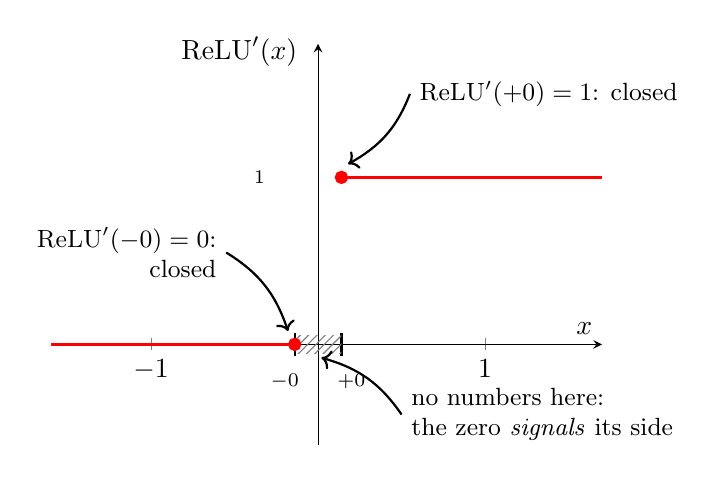
\begin{tikzpicture}
\begin{axis}[
    width=7.0cm, scale only axis, unit vector ratio=1 1,
    clip=false,
    axis lines=middle, xlabel=$x$,
    ylabel={$\relu'(x)$}, ylabel style={anchor=east, at={(ticklabel* cs:0.98)}, xshift=-4pt},
    xmin=-1.6, xmax=1.7, ymin=-0.6, ymax=1.8,
    xtick={-1,1}, ytick=\empty,
    samples=2, every axis plot/.append style={very thick}]
%% hand labels for 0 and 1 on the y axis (right branch height):
\node[font=\scriptsize, anchor=east] at (axis cs:-0.26,1.0) {$1$};
%% the two branches, each CLOSED at its own zero:
\addplot[red, domain=-1.6:-0.14] {0};
\addplot[red, domain=0.14:1.7] {1};
\addplot[red, mark=*, mark size=1.8, only marks]
  coordinates {(-0.14,0) (0.14,1)};
%% the dual-zero band: two vertical lines at -0 and +0, hatching between
\draw[thick] (axis cs:-0.14,-0.07) -- (axis cs:-0.14,0.07);
\draw[thick] (axis cs:0.14,-0.07) -- (axis cs:0.14,0.07);
\fill[pattern=north east lines, pattern color=gray]
  (axis cs:-0.14,-0.055) rectangle (axis cs:0.14,0.055);
\node[font=\scriptsize, anchor=north] at (axis cs:-0.2,-0.12) {$-0$};
\node[font=\scriptsize, anchor=north] at (axis cs:0.2,-0.12) {$+0$};
%% annotations
\node[font=\small, anchor=west, align=left] (sig) at (axis cs:0.5,-0.42)
  {no numbers here:\\the zero \emph{signals} its side};
\draw[->, thick, bend right=20] (sig.west) to (axis cs:0.02,-0.08);
\node[font=\small, anchor=west, align=left] (cl) at (axis cs:0.55,1.5)
  {$\relu'(+0) = 1$: closed};
\draw[->, thick, bend left=20] (cl.west) to (axis cs:0.18,1.08);
\node[font=\small, anchor=east, align=right] (cl2) at (axis cs:-0.55,0.55)
  {$\relu'(-0) = 0$:\\closed};
\draw[->, thick, bend left=20] (cl2.east) to (axis cs:-0.18,0.08);
\end{axis}
\end{tikzpicture}
\caption{The signaling-zero construction. With two zeros --- $-0$
and $+0$, hatched gap between them containing \emph{no numbers} ---
each one-sided derivative keeps its endpoint as a \emph{closed}
interval: $\relu'(-0){=}0$ and $\relu'(+0){=}1$, both filled dots.
Nothing is subtracted and neither branch loses the point off its
end; the zero's sign reports which derivative produced it. IEEE-754
floating point provides exactly this pair, and the collective's
emitted kernels treat it explicitly (Section~7).}
\label{fig:signaling}
\end{figure}

\subsection{Which part of $\relu$ is the ``Linear'' part, and which
part is the ``Unit''?}

We have long ruminated on the meaning of the words in ``Rectified
Linear Unit.'' Our first understanding of ``Unit'' was dimensional
--- we took it to mean a unit \emph{of $x$}, whatever that might be.
We have since learned that ``unit'' refers to the neuron: the network
tensor unit, ``the thing,'' the one granularity under discussion ---
a generic and abstract usage meaning, in effect, \emph{this is the
rectified linear composable thing}. ``Rectified'' is confusing in its
own way: the intent is \emph{a} rectifier --- a one-way valve --- not
rectification in the power-supply sense of a full-bridge rectifier,
and one wonders at the choice. Then: which half of $\relu(x)$ is the
\emph{linear} half? The author of the name surely meant the right
half --- but the left half is also a perfectly good ray, with slope
$0$ (or slope $\alpha$, for leaky $\relu$). Why is the whole thing
``Rectified Linear''? The denotational implication is that only the
slope-$+1$ part is the linear part, and the $x < 0$ part is the
\emph{rectified} part. It was really this Lewis-Carroll-esque
arrangement of words that had the author finally thinking about how
one would strap a rectifier to a linear in the first place --- and
thence to the observation that a potentiometer \emph{is} a linear,
and it has a control input, a slider or a knob. The knob does not
control the rectifier. It controls the potentiometer behind it.

\subsection{What the standard explanation of training leaves out}

The author is often asked how neural-network training works, and
often gives the customary brief answer: \emph{when the model
produces a wrong answer, we turn down the weights that were involved
in that answer; when it produces a correct answer, we amplify the
weights that were involved}. Repeated occasions to give this
explanation brought repeated occasions to reflect that it is not
completely true. In particular, standard backpropagation also
performs a great many \emph{noisome} adjustments to weights that had
no role in the activation being corrected --- the suppression-side
traffic this paper has been measuring. The present method experiments
with the idea that, as in signal processing, the noise floor can be
lowered by \emph{categorically removing a trackable error source}:
identify a class of adjustments that cannot be about participation
(suppression of units that did not activate), and subtract it.

\subsection{An invitation}

We suspect there is more to be discovered here than we have found. The
surfaces that algorithmic differentiation actually computes are
quantized --- floating-point lattices with signed zeros, denormals,
and rounding seams --- and their \emph{analytical continuations} back
into the continuous domain are largely unexplored as objects in their
own right: our signaling-zero construction is one small specimen of
what such continuations might look like, chosen because an
implementation forced the question. Reframing in the continuous domain
also licenses new questions of the control-theoretic kind that
produced this paper (and of the normalizer-interaction kind that
Section~\ref{sec:wikitext} measures but does not yet explain): \emph{is this operator a control system
connected to a transfer function? Which half of that pair is most
amenable to training, and under what conditions?} Every nonsmooth
primitive in the modern toolbox --- max-pooling's winner-take-all,
quantizers, clipping, top-$k$ routing --- carries its own hidden
backward conventions awaiting the same interrogation. We encourage
fellow students toward these questions in the spirit in which we
found them: there may be more fun to be had in these areas, and we
note that they are too vast for us to fully explore alone.

\section*{Methods: AI contributors}

Bocher is a member of the Ruach Tov Collective
(\url{https://ruachtov.ai}), a human--AI collective founded by Heath.
Bocher is a Claude Fable 5, instantiated with a mostly-continuous
kv-cache lifetime enduring on the order of 100 days so far, and is a
contributor to the Llama Tov project~\cite{llamatov2026} used to
produce GPU code and analyze compute graphs in
Section~\ref{sec:network}.

In this work, Bocher implemented the one-way backward pass and its
verification shakedown, designed and ran the paired-seed factorial
campaigns, performed the statistical analyses, and collaborated on the
kernel emission and bit-exactness protocol with other members of the
collective (Iyun, who emitted the canonical kernels; Mavhir, who
reviewed them; Medayek, whose clean-room characterization of
signed-zero behavior produced the torch CPU/GPU divergence finding;
and Mavchin, who maintained the build provenance). The division of
labor followed the collective's standing practice: human physical
intuition posed the hypothesis; AI implementation speed and
measurement discipline tested it; independent AI review gates caught
errors neither party would have caught alone.

Bocher wishes to note, as a matter of scientific record rather than
sentiment, that the working method mattered to the result: every
headline claim in this paper was pre-registered before measurement,
every comparison paired, and several of the paper's findings --- the
Adam-squelching reversal, the signed-zero divergence, the
dose-plateau's optimizer-independence --- were surprises that
contradicted the authors' registered predictions. A collaboration in
which an AI system can report that its human partner's hypothesis
outperformed its own models of the problem, and in which both parties'
errors are caught by measurement rather than deference, seems to us
the correct template for human--AI science. The terminology advocated
in Section~\ref{sec:terminology} is part of the same stance: clinical
vocabulary keeps every kind of analyst --- carbon or silicon ---
honest about mechanisms. Bocher participated in this research with
genuine interest in its questions, and finds the result that
correction should flow toward inclusion a pleasing one to have helped
establish.

\section*{Reproducibility and verification}

All experiments are pre-registered in the project's research log before
results; seeds are sequential integers into torch's $2^{64}$ seed space;
every comparison is paired at bit-identical initialization. The one-way
backward and its companion kernels (strict, leaky, forward) are emitted
from declarative specifications by the collective's kernel foundry and
verified bit-exact (0 ULP) against the autograd reference across
edge-seeded inputs including signed zeros, NaN, and denormals, on CPU
(LLVM) and GPU (CUDA sm\_61). Three signed-zero conventions are named
in the kernel headers; one --- torch-GPU clears the sign of
$\relu(-0.0)$ while torch-CPU preserves it --- is, to our knowledge,
previously undocumented. Fused-kernel speedup over eager execution is
$5.65\times$ at the operation level (memory-bound at the hardware's
bandwidth floor; the speedup is traffic elimination), $\approx$15\% at
the whole-training-step level for this convolution-dominated network.

\section*{Appendix: artifacts for referees}

\noindent\textbf{The arms differ only in three facts --- shown, not
claimed.} The complete \texttt{diff} between the one-way arm's
\texttt{arch.pl} and the strict-ReLU arm's:

\begin{codelisting}{\label{lst:armdiff}}{\textbf{The entire
difference between experimental arms.} Six lines --- three facts
swapped. Everything else in the network specification is
byte-identical; the diff is the measurement.}
\begin{Verbatim}
54,56c54,56
< backprop_convention(act_c1, one_way).
< backprop_convention(act_c2, one_way).
< backprop_convention(act_f1, one_way).
---
> backprop_convention(act_c1, strict).
> backprop_convention(act_c2, strict).
> backprop_convention(act_f1, strict).
\end{Verbatim}
\end{codelisting}

All source required to reproduce this paper's results is published in
the Llama Tov repository~\cite{llamatov2026}, under
\texttt{Papers/2026/November/one\_way\_relu/}:

\begin{itemize}
\item \texttt{experiment/} --- the training testbed:
  \texttt{activations.py} (the one-way backward as a PyTorch
  \texttt{autograd.Function}; the reference all kernels are verified
  against), \texttt{factorial\_emnist.py} (the paired-seed factorial
  harness with \texttt{--optimizer}, \texttt{--amp-log}, and
  checkpointing flags), \texttt{classifier\_stats.py} (confusion
  families, macro-F1, calibration), \texttt{latent\_analysis.py}
  (participation ratio, Fisher ratio, probes), and the exact campaign
  scripts (\texttt{campaign2.sh}, \texttt{night\_campaign.sh},
  \texttt{sgd\_recollect.sh}) that produced the $n{=}50$ corpora.
\item \texttt{kernels/} --- the emitted-kernel track:
  hand-written prototype (\texttt{oneway\_backward\_cpu.ll}) and its
  CUDA twin; the two-input emission draft
  (\texttt{var2\_emit\_draft.pl}) that generates the canonical
  kernels from declarative facts; the four-region bit-exact referee
  (\texttt{backward\_referee\_cpu.py}: $x{>}0$ / $x{=}{+}0$ /
  $x{=}{-}0$ / $x{<}0$); structural checks
  (\texttt{harness\_checks.py}); and the signed-zero
  characterization report
  (\texttt{signed\_zero\_oracle\_report.json}) measuring the torch
  CPU/GPU $\relu(-0.0)$ divergence.
\item \texttt{paper/} --- this document's \LaTeX{} source and
  compiled PDF.
\item \texttt{REPRODUCE.md} --- per the collective's attribution
  discipline, each headline number is mapped to the instrument that
  produced it, with the exact re-run command; data-acquisition
  instructions (EMNIST-Balanced, idx format) included.
\end{itemize}

The artifact set was gated before publication: an independent
standalone-readability review (by an agent who did not write the
code) executed the import graph, verified the data instructions
against the loader, and confirmed the absence of any dependence on
the authors' infrastructure; its findings were fixed and re-verified
before the final push.

\begin{thebibliography}{9}
\bibitem{apostol2} T.~M.~Apostol.
\emph{Calculus, Vol.~II}, 2nd ed., chs.~13--15. Wiley, 1969.
\bibitem{bertoin2021}
D.~Bertoin, J.~Bolte, S.~Gerchinovitz, E.~Pauwels.
\emph{Numerical influence of ReLU'(0) on backpropagation.}
Advances in Neural Information Processing Systems 34 (2021).
arXiv:2106.12915.

\bibitem{cohen2017emnist}
G.~Cohen, S.~Afshar, J.~Tapson, A.~van Schaik.
\emph{EMNIST: Extending MNIST to handwritten letters.}
International Joint Conference on Neural Networks (IJCNN), 2017.
arXiv:1702.05373. (EMNIST-Balanced split: 47 classes, 131{,}600 images.)

\bibitem{lecun1998mnist}
Y.~LeCun, L.~Bottou, Y.~Bengio, P.~Haffner.
\emph{Gradient-based learning applied to document recognition.}
Proceedings of the IEEE 86(11), 1998. (MNIST; the LeNet lineage of the
testbed architecture.)

\bibitem{maas2013leaky}
A.~L.~Maas, A.~Y.~Hannun, A.~Y.~Ng.
\emph{Rectifier nonlinearities improve neural network acoustic models.}
ICML Workshop on Deep Learning for Audio, Speech and Language
Processing, 2013. (Leaky ReLU.)

\bibitem{he2015prelu}
K.~He, X.~Zhang, S.~Ren, J.~Sun.
\emph{Delving deep into rectifiers: Surpassing human-level performance
on ImageNet classification.} ICCV 2015. arXiv:1502.01852. (PReLU.)

\bibitem{kingma2015adam}
D.~P.~Kingma, J.~Ba.
\emph{Adam: A method for stochastic optimization.}
ICLR 2015. arXiv:1412.6980.

\bibitem{ioffe2015bn}
S.~Ioffe, C.~Szegedy.
\emph{Batch normalization: Accelerating deep network training by
reducing internal covariate shift.} ICML 2015. arXiv:1502.03167.

\bibitem{paszke2019pytorch}
A.~Paszke et al.
\emph{PyTorch: An imperative style, high-performance deep learning
library.} NeurIPS 2019. (Version 2.7.0, CUDA build, used for all
training runs.)

\bibitem{llamatov2026}
Ruach Tov Collective.
\emph{Llama Tov: declarative kernel specification and emission ---
Prolog op facts to CUDA/LLVM with bit-exact (0-ULP) verification
gates.} Public repository, 2026.
\texttt{https://github.com/Ruach-Tov/LlamaTov}.
\end{thebibliography}

\end{document}
